\documentclass[tikz,border=3pt]{standalone}
\usepackage[utf8]{inputenc}
\usepackage[T1]{fontenc}
\usepackage{lmodern}
\renewcommand{\familydefault}{\sfdefault}
\usepackage{sansmath}\sansmath
\usepackage{chemfig}
\usepackage{pgfplots}\pgfplotsset{compat=1.18,/pgf/number format/use comma,/pgf/number format/1000 sep={.}}
\usetikzlibrary{arrows.meta,calc,positioning,decorations.pathmorphing,patterns}
% paleta del sitio
\definecolor{nar}{HTML}{E8680C}\definecolor{narc}{HTML}{FFB35C}\definecolor{hielo}{HTML}{FFF3E8}
\definecolor{tinta}{HTML}{1D1D1F}\definecolor{gris}{HTML}{6E6E73}\definecolor{lila}{HTML}{7C5CF0}
\definecolor{azul}{HTML}{2F6FD6}\definecolor{menta}{HTML}{17A673}\definecolor{coral}{HTML}{E8342A}
\begin{document}
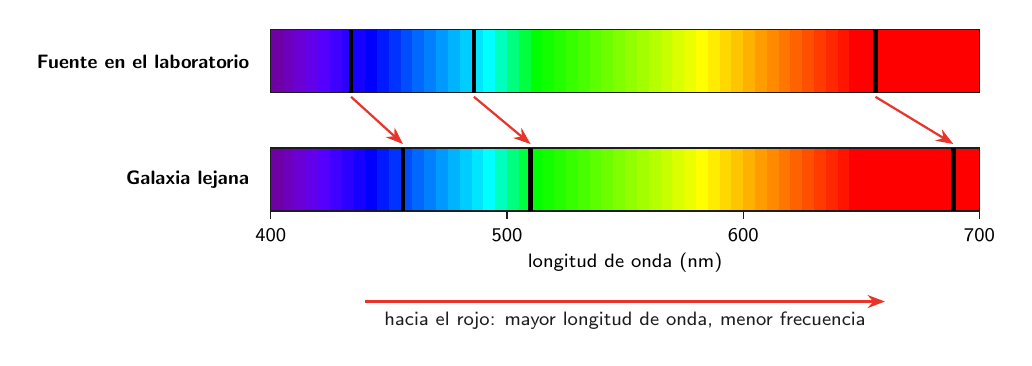
\begin{tikzpicture}[font=\footnotesize,>={Stealth[length=2.2mm]}]
\def\sx{0.03}% cm por nm
\foreach \y/\lab in {1.5/Fuente en el laboratorio, 0/Galaxia lejana}{
  \foreach \l in {400,405,...,695}{
    \definecolor{tmp}{wave}{\l}
    \fill[tmp] ({(\l-400)*\sx},\y) rectangle ({(\l-395)*\sx+0.005},\y+0.8);
  }
  \draw[tinta] (0,\y) rectangle ({300*\sx},\y+0.8);
  \node[anchor=east,font=\scriptsize\bfseries,align=right] at (-0.15,\y+0.4) {\lab};
}
\foreach \l in {434,486,656} \draw[black,line width=1.6pt] ({(\l-400)*\sx},1.5) -- ({(\l-400)*\sx},2.3);
\foreach \l in {456,510,689} \draw[black,line width=1.6pt] ({(\l-400)*\sx},0) -- ({(\l-400)*\sx},0.8);
\foreach \a/\b in {434/456,486/510,656/689} \draw[->,coral,thick] ({(\a-400)*\sx},1.45) -- ({(\b-400)*\sx},0.85);
\foreach \l in {400,500,600,700} {\draw[tinta] ({(\l-400)*\sx},0) -- ({(\l-400)*\sx},-0.1); \node[below,font=\scriptsize] at ({(\l-400)*\sx},-0.1) {\l};}
\node[font=\scriptsize] at ({150*\sx},-0.65) {longitud de onda (nm)};
\draw[->,thick,coral] ({40*\sx},-1.15) -- ({260*\sx},-1.15) node[midway,below,font=\scriptsize,text=tinta] {hacia el rojo: mayor longitud de onda, menor frecuencia};
\end{tikzpicture}
\end{document}
